\documentclass[]{article}
\usepackage{lmodern}
\usepackage{amssymb,amsmath}
\usepackage{ifxetex,ifluatex}
\usepackage{fixltx2e} % provides \textsubscript
\ifnum 0\ifxetex 1\fi\ifluatex 1\fi=0 % if pdftex
  \usepackage[T1]{fontenc}
  \usepackage[utf8]{inputenc}
\else % if luatex or xelatex
  \ifxetex
    \usepackage{mathspec}
  \else
    \usepackage{fontspec}
  \fi
  \defaultfontfeatures{Ligatures=TeX,Scale=MatchLowercase}
\fi
% use upquote if available, for straight quotes in verbatim environments
\IfFileExists{upquote.sty}{\usepackage{upquote}}{}
% use microtype if available
\IfFileExists{microtype.sty}{%
\usepackage{microtype}
\UseMicrotypeSet[protrusion]{basicmath} % disable protrusion for tt fonts
}{}
\usepackage[margin=1in]{geometry}
\usepackage{hyperref}
\hypersetup{unicode=true,
            pdftitle={Oregon Extended Analyses: 2019},
            pdfauthor={Brock Rowley; Sevrina Tindal; Philip Irvin; Daniel Anderson; Gerald Tindal},
            pdfborder={0 0 0},
            breaklinks=true}
\urlstyle{same}  % don't use monospace font for urls
\usepackage{color}
\usepackage{fancyvrb}
\newcommand{\VerbBar}{|}
\newcommand{\VERB}{\Verb[commandchars=\\\{\}]}
\DefineVerbatimEnvironment{Highlighting}{Verbatim}{commandchars=\\\{\}}
% Add ',fontsize=\small' for more characters per line
\usepackage{framed}
\definecolor{shadecolor}{RGB}{248,248,248}
\newenvironment{Shaded}{\begin{snugshade}}{\end{snugshade}}
\newcommand{\AlertTok}[1]{\textcolor[rgb]{0.94,0.16,0.16}{#1}}
\newcommand{\AnnotationTok}[1]{\textcolor[rgb]{0.56,0.35,0.01}{\textbf{\textit{#1}}}}
\newcommand{\AttributeTok}[1]{\textcolor[rgb]{0.77,0.63,0.00}{#1}}
\newcommand{\BaseNTok}[1]{\textcolor[rgb]{0.00,0.00,0.81}{#1}}
\newcommand{\BuiltInTok}[1]{#1}
\newcommand{\CharTok}[1]{\textcolor[rgb]{0.31,0.60,0.02}{#1}}
\newcommand{\CommentTok}[1]{\textcolor[rgb]{0.56,0.35,0.01}{\textit{#1}}}
\newcommand{\CommentVarTok}[1]{\textcolor[rgb]{0.56,0.35,0.01}{\textbf{\textit{#1}}}}
\newcommand{\ConstantTok}[1]{\textcolor[rgb]{0.00,0.00,0.00}{#1}}
\newcommand{\ControlFlowTok}[1]{\textcolor[rgb]{0.13,0.29,0.53}{\textbf{#1}}}
\newcommand{\DataTypeTok}[1]{\textcolor[rgb]{0.13,0.29,0.53}{#1}}
\newcommand{\DecValTok}[1]{\textcolor[rgb]{0.00,0.00,0.81}{#1}}
\newcommand{\DocumentationTok}[1]{\textcolor[rgb]{0.56,0.35,0.01}{\textbf{\textit{#1}}}}
\newcommand{\ErrorTok}[1]{\textcolor[rgb]{0.64,0.00,0.00}{\textbf{#1}}}
\newcommand{\ExtensionTok}[1]{#1}
\newcommand{\FloatTok}[1]{\textcolor[rgb]{0.00,0.00,0.81}{#1}}
\newcommand{\FunctionTok}[1]{\textcolor[rgb]{0.00,0.00,0.00}{#1}}
\newcommand{\ImportTok}[1]{#1}
\newcommand{\InformationTok}[1]{\textcolor[rgb]{0.56,0.35,0.01}{\textbf{\textit{#1}}}}
\newcommand{\KeywordTok}[1]{\textcolor[rgb]{0.13,0.29,0.53}{\textbf{#1}}}
\newcommand{\NormalTok}[1]{#1}
\newcommand{\OperatorTok}[1]{\textcolor[rgb]{0.81,0.36,0.00}{\textbf{#1}}}
\newcommand{\OtherTok}[1]{\textcolor[rgb]{0.56,0.35,0.01}{#1}}
\newcommand{\PreprocessorTok}[1]{\textcolor[rgb]{0.56,0.35,0.01}{\textit{#1}}}
\newcommand{\RegionMarkerTok}[1]{#1}
\newcommand{\SpecialCharTok}[1]{\textcolor[rgb]{0.00,0.00,0.00}{#1}}
\newcommand{\SpecialStringTok}[1]{\textcolor[rgb]{0.31,0.60,0.02}{#1}}
\newcommand{\StringTok}[1]{\textcolor[rgb]{0.31,0.60,0.02}{#1}}
\newcommand{\VariableTok}[1]{\textcolor[rgb]{0.00,0.00,0.00}{#1}}
\newcommand{\VerbatimStringTok}[1]{\textcolor[rgb]{0.31,0.60,0.02}{#1}}
\newcommand{\WarningTok}[1]{\textcolor[rgb]{0.56,0.35,0.01}{\textbf{\textit{#1}}}}
\usepackage{graphicx,grffile}
\makeatletter
\def\maxwidth{\ifdim\Gin@nat@width>\linewidth\linewidth\else\Gin@nat@width\fi}
\def\maxheight{\ifdim\Gin@nat@height>\textheight\textheight\else\Gin@nat@height\fi}
\makeatother
% Scale images if necessary, so that they will not overflow the page
% margins by default, and it is still possible to overwrite the defaults
% using explicit options in \includegraphics[width, height, ...]{}
\setkeys{Gin}{width=\maxwidth,height=\maxheight,keepaspectratio}
\IfFileExists{parskip.sty}{%
\usepackage{parskip}
}{% else
\setlength{\parindent}{0pt}
\setlength{\parskip}{6pt plus 2pt minus 1pt}
}
\setlength{\emergencystretch}{3em}  % prevent overfull lines
\providecommand{\tightlist}{%
  \setlength{\itemsep}{0pt}\setlength{\parskip}{0pt}}
\setcounter{secnumdepth}{0}
% Redefines (sub)paragraphs to behave more like sections
\ifx\paragraph\undefined\else
\let\oldparagraph\paragraph
\renewcommand{\paragraph}[1]{\oldparagraph{#1}\mbox{}}
\fi
\ifx\subparagraph\undefined\else
\let\oldsubparagraph\subparagraph
\renewcommand{\subparagraph}[1]{\oldsubparagraph{#1}\mbox{}}
\fi

%%% Use protect on footnotes to avoid problems with footnotes in titles
\let\rmarkdownfootnote\footnote%
\def\footnote{\protect\rmarkdownfootnote}

%%% Change title format to be more compact
\usepackage{titling}

% Create subtitle command for use in maketitle
\providecommand{\subtitle}[1]{
  \posttitle{
    \begin{center}\large#1\end{center}
    }
}

\setlength{\droptitle}{-2em}

  \title{Oregon Extended Analyses: 2019}
    \pretitle{\vspace{\droptitle}\centering\huge}
  \posttitle{\par}
    \author{Brock Rowley \\ Sevrina Tindal \\ Philip Irvin \\ Daniel Anderson \\ Gerald Tindal}
    \preauthor{\centering\large\emph}
  \postauthor{\par}
      \predate{\centering\large\emph}
  \postdate{\par}
    \date{6/29/2019}

\pagenumbering{gobble}
\usepackage{placeins}
\usepackage{float}
\usepackage{caption}
\captionsetup[figure]{labelformat = empty}
\usepackage{xcolor}
\definecolor{link}{rgb}{0, 0, 238}
\usepackage{booktabs}

\begin{document}
\maketitle

{
\setcounter{tocdepth}{5}
\tableofcontents
}
\hypertarget{oregon-department-of-education}{%
\section{Oregon Department of
Education}\label{oregon-department-of-education}}

\hypertarget{technical-report}{%
\section{2018-2019 Technical Report}\label{technical-report}}

\hypertarget{oregons-alternate-assessment-system}{%
\subsection{Oregon's Alternate Assessment
System}\label{oregons-alternate-assessment-system}}

\hypertarget{peer-review-documentation-critical-elements-1-6}{%
\subsection{Peer Review Documentation: Critical Elements
1-6}\label{peer-review-documentation-critical-elements-1-6}}

\hypertarget{oregons-alternate-assessment-system-technical-report}{%
\subsubsection{Oregon's Alternate Assessment System Technical
Report:}\label{oregons-alternate-assessment-system-technical-report}}

\hypertarget{peer-review-documentation-critical-elements-1-6-1}{%
\subsubsection{Peer Review Documentation: Critical Elements
1-6}\label{peer-review-documentation-critical-elements-1-6-1}}

It is the policy of the State Board of Education and a priority of the
Oregon Department of Education that there will be no discrimination or
harassment on the grounds of race, color, religion, sex, sexual
orientation, national origin, age or disability in any educational
programs, activities or employment. Persons having questions about equal
opportunity and nondiscrimination should contact the Deputy
Superintendent of Public Instruction with the Oregon Department of
Education.

\emph{This technical report is one of a series that describes the
development of Oregon's Statewide Assessment System. The complete set of
volumes provides comprehensive documentation of the development,
procedures, technical adequacy, and results of the system.}

\newpage

\includegraphics{Figures/peer_rev/PeerReview1.pdf}

\newpage

\includegraphics{Figures/peer_rev/PeerReview2.pdf}

\newpage

\includegraphics{Figures/peer_rev/PeerReview3.pdf}

\newpage

\includegraphics{Figures/peer_rev/PeerReview4.pdf}

\newpage

\includegraphics{Figures/peer_rev/PeerReview5.pdf}

\newpage

\includegraphics{Figures/peer_rev/PeerReview6.pdf}

\hypertarget{overview}{%
\section{Overview}\label{overview}}

This document provides updated technical adequacy documentation for the
Oregon Extended Assessment (ORExt), which is Oregon's alternate
assessment based on alternate academic achievement standards (AA-AAAS).
The documentation includes test design and development, technical
characteristics of the assessments, and their uses, and impact in
providing proficiency data on grade level state standards as part of the
mandates from the Every Student Succeeds Act of 2015 (ESSA).

The ORExt assessments were redesigned in 2014-15, including a vertical
scale in Grades 3-8 in English language arts and mathematics to support
eventual determinations of student growth over time. The test is aligned
to Essentialized Standards (EsSt) that are part of comprehensive
Essentialized Assessment Frameworks (EAFs) that were written at three
levels of complexity (low, medium, and high). The EsSt have been linked
to grade level content and expectations, but systematically reduced in
terms of depth, breadth, and complexity (RDBC). All ORExt items employed
in the 2018-19 ORExt administration, with the exception of Grade 7 Math
field test items, were developed in 2014-15. Based on student
performance from the 2016-2017 testing year, new and Grade 7 Math field
test items were written in fall 2017.

A statewide sample of Oregon general and special education teachers have
reviewed all test items for: 1) alignment to the EAFs, 2) accessibility
for students with significant cognitive disabilities, 3) sensitivity,
and 4) bias. All operational items met the established criteria. In
addition, Achievement Level Descriptors (ALDs) were also reviewed for
alignment to the EsSt. See Sections 1.1, 1.2, 6.1, and 6.3 for
additional information related to the comprehensive grade level
standards to EsSt linkage, as well as alignment of items to the EsSt.

The ORExt test design supports student access, including access to read
aloud for directions and prompts, presentation of one item per page, and
items designed at three levels of complexity where the low level
complexity items include graphic and/or object support. For assessors,
the scoring process has also been simplified, with answers being either
correct (1) or incorrect (0). Partial credit is no longer part of the
scoring metric for the ORExt. In addition, the one item per page format
not only increases student ability to focus attention, but also reduces
the burden on assessors to mask items that are not being tested. The
field appears to have been appreciative of the redesign, particularly
the Essentialized Standards and new access and efficiency features.

In addition to developing and reviewing/editing over 5,000 new items,
conducting an operational field test, and developing a vertical scale,
the development of a new ORExt required that new Alternate Academic
Achievement Standards (AAAAS) be developed and approved. Comprehensive
Standard Setting meetings were conducted on June 15-17, 2015, which were
then approved by the Oregon State Board of Education on June 25, 2015,
including new achievement level descriptors (ALDs) and cut scores for
the assessments. Comprehensive Annual Measurable Objective (AMO) reports
were finalized on July 10, 2015.

Though an alignment study was conducted in the fall of 2014 as described
above, Non-Regulatory Guidance from the U.S. Department of Education,
published on September 25, 2015, included an expectation that all
alignment studies must be independent (see Critical Element 3.1). An
independent contractor, Dr.~Dianna Carrizales, was therefore hired to
perform an additional alignment study in the spring of 2017.

A two year pilot tablet study was conducted in the 2015-2016 and 2016-17
school years. Over the two year study, 26 students were administered all
subject areas of the ORExt in tablet format in grades 5, 8, and 11. The
2017-18 school year marked the first year the ORExt was available in
tablet/online format for all grades in all subject areas.

As part of our five-year technical documentation plan, which included
the independent alignment study, pilot tablet administration study, and
launch of the full tablet administration, an inter-rater reliability
study was also conducted in 2017-18. The inter-rater reliability study
included 33 Qualified Trainers from around the state who participated by
doing at least one Qualified Assessor observation on the Oregon Extended
Assessment via paper/pencil administration. As part of the five-year
plan, following the 2018-19 test administration, an analyses of the
impact of accommodations was conducted.

\hypertarget{r-markdown}{%
\subsection{R Markdown}\label{r-markdown}}

This is an R Markdown document. Markdown is a simple formatting syntax
for authoring HTML, PDF, and MS Word documents. For more details on
using R Markdown see \url{http://rmarkdown.rstudio.com}.

When you click the \textbf{Knit} button a document will be generated
that includes both content as well as the output of any embedded R code
chunks within the document. You can embed an R code chunk like this:

\begin{Shaded}
\begin{Highlighting}[]
\KeywordTok{summary}\NormalTok{(cars)}
\end{Highlighting}
\end{Shaded}

\begin{verbatim}
##      speed           dist       
##  Min.   : 4.0   Min.   :  2.00  
##  1st Qu.:12.0   1st Qu.: 26.00  
##  Median :15.0   Median : 36.00  
##  Mean   :15.4   Mean   : 42.98  
##  3rd Qu.:19.0   3rd Qu.: 56.00  
##  Max.   :25.0   Max.   :120.00
\end{verbatim}

\hypertarget{including-plots}{%
\subsection{Including Plots}\label{including-plots}}

You can also embed plots, for example:

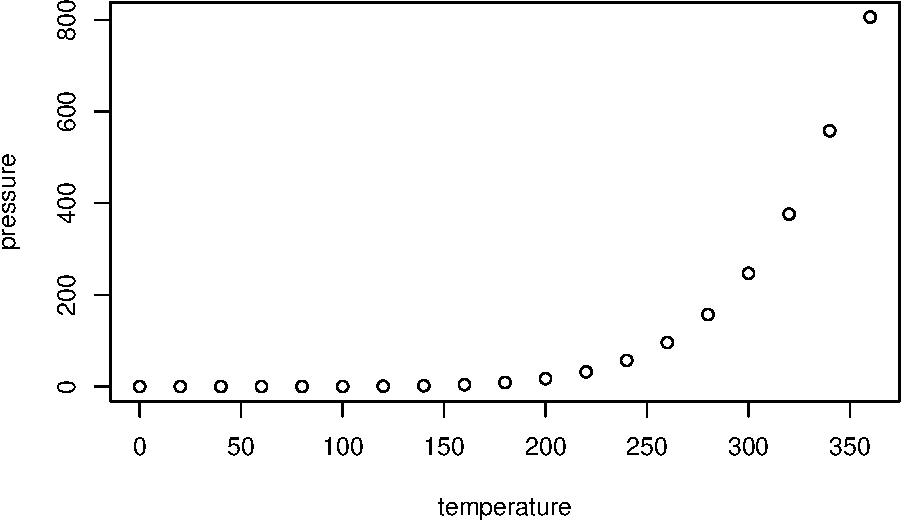
\includegraphics{ORExt_Intro_files/figure-latex/pressure-1.pdf}

Note that the \texttt{echo\ =\ FALSE} parameter was added to the code
chunk to prevent printing of the R code that generated the plot.


\end{document}
